\documentclass[a4paper,12pt]{article}
\usepackage[ngerman]{babel}
\usepackage{ucs}
\usepackage{multirow}
\usepackage{xltxtra}
\usepackage[utf8x]{inputenc}
\usepackage{fontspec}
\usepackage[automark]{scrpage2}
\usepackage{eurosym}
\usepackage{graphicx}
\usepackage[paper=a4paper,left=25mm,right=25mm,top=25mm,bottom=25mm]{geometry}
\pagestyle{scrheadings}
\setmainfont[Mapping=tex-text]{Liberation Serif}
\clearscrheadfoot
\ohead{Regelstand: \today}
\title{2020 SUMO Challenge Regeln}
\makeatletter
\let\inserttitle\@title
\makeatother

\begin{document}

 \begin{center}

\includegraphics[width=0.5\textwidth]{logo.png}

\huge                      % Schriftgröße einstellen
\bfseries                   % Fettdruck einschalten
\inserttitle
  \end{center}
  %Inhaltliche Änderungen im Vergleich zu den Regeln von 2017 sind \textbf{fett} markiert. Im Zweifel ist die Interpretation der Regeln durch die Schiedsrichter bindend.
\section{Aufgabe}
Entwerfe, baue und programmiere einen autonomen Sumo-Roboter, der einen oder mehrere gegnerische Sumo-Roboter von einem erhöhten Wrestling-Ring stoßen kann. Das Gewicht eines SumoBots ist abhängig von der Altersgruppe.

% Überschrift ändern?
\section{Wer kann teilnehmen? / Altersgruppe}
Bitte entnehmen Sie der untenstehenden Tabelle, in welcher Division/Massenklasse Sie teilnehmen möchten.
\begin{center}
\begin{tabular}{|c|c|c|} \hline
	\multirow{2}*{1kg} & \multirow{2}*{2kg} & Lego Only 1Kg \\
	& & (Optional) \\ \hline
	%ES &  & ES \\ \hline
	%MS & ** & MS \\ \hline
	MS & MS & MS \\ \hline
	HS & HS & HS \\ \hline
	%** & UP & ** \\ \hline
\end{tabular} \\ \vspace{\baselineskip}
\end{center}

% Dies sind die Klassen aus den Regeln 2019
%	Klasse 			&& Altersgruppe 			&& Gewicht
%	Mini SumoBot		&& 0					&&	1kg
%	Medium SumoBot	&& 1 (Middle School): 10-13 Jahre	&&	2kg
%	Mega SumoBot		&& 2 (High School/) : 14-17 Jahre	&&	3kg


\section{Roboter}
%\section{Materialanforderungen}
% Autonomer Roboter basierend auf jeglicher Plattform, der maximal EUR 1500 kostet und den folgenden Designanforderungen, die beim Check-In überprüft werden, entspricht:
Autonomer Roboter, jede beliebige Plattform, die 1.500 USD oder weniger kostet und die folgenden Designbeschränkungen erfüllt, die beim Robot Check-In überprüft werden.
\begin{itemize}
	\item Die maximale Größe des Roboters beträgt 25 cm x 18 cm ohne Höhenbeschränkung, gemessen mit allen beweglichen Komponenten in ihrer Ausgangsposition.
	\item Die Roboterklasse wird beim Check-In überprüft
	\item Der Roboter kann die Kante des Rings vermeiden und seine Gegner suchen. Er in der Lage ist den Sumo-Ring von einer gegebenen Startposition zu navigieren.
	\item Nur Teammitglieder dürfen den Roboter entwickeln, konstruieren und programmieren.
	%\item Das Volumen des Roboters darf 400 cm^3 nicht überschreiten.
\end{itemize}

\section{Aufgabenbeschreibung}
\subsection{Roboter Einschränkungen (Verboten)}

\begin{itemize}
	\item Störgeräte, wie Infrarot-LEDs, die dazu benutzt werden den gegnerischen Infrarotsensor zu sättigen/übersteuern. % Ändern?
	\item Teile die den Ring oder den/die Roboter beschädigen oder Zerstören könnten.
	\item Teile deren Zweck die Beschädigung oder Zerstörung des gegnerischen Roboters ist. Normales Schieben oder Stoßen werden nicht als absichtliche Beschädigung gewertet.
	\item Vorrichtungen die Flüssigkeiten, Puder, Gas oder andere Substanzen enthalten, um sie auf den Gegner zu werfen.
	\item Klebrige Substanzen oder Klebstoffe, um die Bodenhaftung zu erhöhen.
	\item Vorrichtungen, um die Bodenhaftung zu erhöhen, wie Magnete und Vakuumpumpen.
	\item Scharfen Kanten (Es zählen alle Kanten, die leicht Haut verletzen können)
\end{itemize}

\subsection{Ring Spezifikationen}
\begin{itemize}
	\item Ein etwa ~122cm im Durchmesser weißer runder Bereich mit einer ~5cm dicken schwarzen Kante.
	\item Der Sumo-Ring wird mit etwa 1.25 cm dickem Sperrholz oder andere passende nicht magnetische Materialien konstruiert.
	\item Der Sumo-Ring soll mit an der Unterseite des Rings angebrachten Stützbalken um etwa ~2.54 cm vom Boden erhöht werden. Diese Stützen müssen mindestens 1cm von der Oberkante des Rings entfernt sein. % andere Maße?
\end{itemize}

\subsection{Platzierung des Roboters}
\begin{itemize}
	\item Jeweils drei Stellen der Kante des Ringes werden farblich markiert. Die Länge der Markierung beträgt etwa 20 cm und ist jeweils um 120° verschoben.
	\item Nach den Instruktionen des Schiedsrichters, werden die Roboter auf dem Ring an eine farbige Markierung gestellt.
	\item Roboter müssen mit der Vorderseite nach außen (vom Zentrum des Rings gesehen) aufgestellt werden. Sie sollen leicht über die innere Kante des schwarzen Ringes hinausragen.
\end{itemize}

% TODO: besseres Bild?
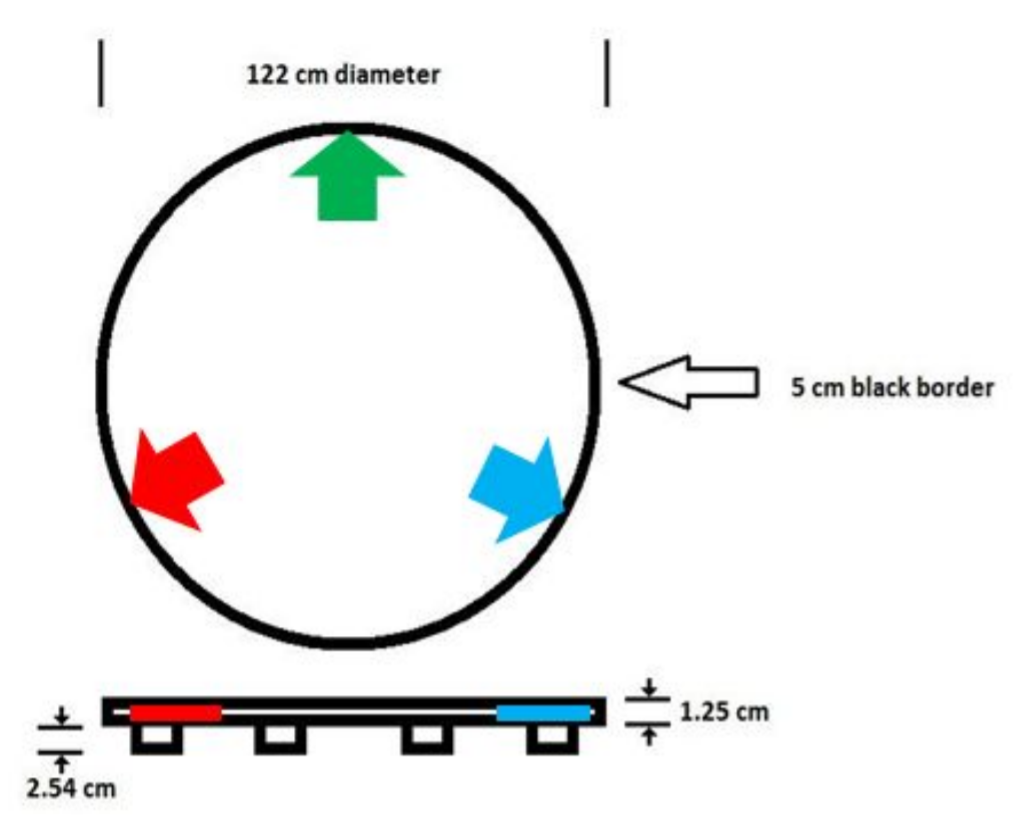
\includegraphics[width=0.8\textwidth]{sumo_bot_ring.png}

\section{Generelle Spielregeln}
\begin{itemize}
	\item SumoBot Spiele sind schnell und enden oft in einem Unentschieden. Jedes Team erhält eine Spiel-Karte für bis zu 25 Spiel. Die 10 besten Spiele ergeben den Punktestand.
	\item Während der Punktephase wird jedem Team am Schiedsrichtertisch der Sumo-Ring für das nächste Spiel bekannt gegeben.
	\item Es wird versucht immer drei Teams pro Spiel antreten zu lassen. Wenn dies nicht möglich ist, können aber auch nur 2 Teams antreten. (Die maximal erzielbaren Punkte reduzieren sich auf 3) % 2 oder 3 Punkte?
	\item Wenn zwei SumoBots fast gleichzeitig herunterfallen, gewinnt der Roboter, der zuletzt den Boden berührt hat. Dies wird vom Schiedsrichter bestimmt und es werden dementsprechend Punkte vergeben.
	\item Nur ein Teammitglied darf am Ring den Roboter starten. Die restlichen Teammitglieder müssen sich mit etwas Entfernung hinter dem eigenen SumoBot aufstellen.
	\item Jedes Team tritt mit einem Roboter an, den das Team selbst nach den Spezifikationen dieses Dokumentes konstruiert hat.
	\item Das Spiel startet mit dem Zeichen des Schiedsrichters und dauert eine Minute oder bis nur noch ein SumoBot im Ring steht.
	\item Wenn sich die Roboter innerhalb eines Zeitraums von 5 Sekunden nicht oder kaum bewegt haben (ein Patt), wird die Uhr angehalten. Die Roboter werden zurück auf die Startposition gestellt und das Spiel wird mit der verbleibenden Zeit weitergeführt. Das Einschätzen eines Patts liegt im Ermessen des Schiedsrichters.
	\item Die Entscheidungen des Schiedsrichters sind endgültig und entscheiden den Sieger des Spiels.
	\item SumoBots die vom Spielrand gestoßen wurden sind aus dem laufenden Spiel ausgeschieden.
\end{itemize}

\section{Punkteermittlung}
\begin{itemize}
	\item Teams sammeln innerhalb eines Spiels zwischen 0 bis 4 Punkte. Die maximale Punktzahl in einem Spiel mit 2 SumoBots ist 3 und mit 3 SumoBots 4.
	\item Jedes Mal, wenn ein SumoBot vom Rand des Ringes gestoßen wurde wird ein Punkt vergeben. Wenn zwei SumoBots in physischen Kontakt stehen und der dritte über die Kante gestoßen wird, erhalten beide verbleibenden Roboter einen Punkt.
	\item Wenn nur ein Roboter im Ring verbleibt, bekommt er einen Punkt für das stehen im Ring und einen Bonuspunkt für das vorzeitige beenden des Spiels.
	\item Wenn das Spiel endet erhalten alle im Ring verbleibenden Roboter einen Punkt.
	\item Das Spiel wird angehalten und mit der verbleibenden Zeit neugestartet, wenn folgende Bedingungen erfüllt sind:
	\begin{itemize}
		\item Die verbleibenden SumoBots bewegen sich kaum oder nicht (ein Patt) innerhalb einer Zeit von 5 Sekunden
		\item Wenn es nicht klar ist ob weitere Fortschritte nach Ablauf der Zeit erzielt werden, kann der Schiedsrichter das Spiel für bis zu 15 Sekunden verlängern.
	\end{itemize}
	\item Die 9 SumoBot-Teams mit dem höchsten Punktestand werden im finalen Wettkampf gegeneinander antreten.
\end{itemize}

\section{Wettkampf Punkteermittlung}
% TODO: Überschriften ändern?

Die top neun Teams werden in drei Gruppen eingeteilt wo sie in einem drei Runden Wettkampf antreten.

Runde Eins: Jedes Team kämpft bis ein SumoBot aus dem Ring gestoßen wurde.
\begin{enumerate}
	\item  Die Verlierer SumoBots aus den drei Kämpfen werden eliminiert
	\item  Der siebte, achte und neunte Platz wird anhand der Gesamtpunktzahl der eliminierten SumoBots bestimmt.
\end{enumerate}

Runde Zwei: Die verbleibenden sechs Teams kämpfen bis ein Sumobot aus dem Ring gestoßen wurde.
\begin{enumerate}
	\item Die Verlierer SumoBots aus den zwei Kämpfen werden eliminiert.
	\item Der fünfte und sechste Platz wird anhand der Gesamtpunktzahl der eliminierten SumoBots bestimmt.
\end{enumerate}

Runde Drei: Die verbleibenden vier Teams kämpfen in einem alles oder nichts SumoBot Showdown. Die Roboter werden dabei jeweils in 90 Grad Intervallen im Ring aufgestellt.
 \begin{enumerate}
	 \item Vierter Platz für den ersten SumoBot der aus dem Ring gestoßen wurde
	 \item Dritter Platz für den zweiten SumoBot der aus dem Ring gestoßen wurde
	 \item Zweiter Platz für den dritten SumoBot der aus dem Ring gestoßen wurde
	 \item Der als letztes stehende SumoBot ist der Champion!
 \end{enumerate}

\end{document}
